\documentclass[conference]{IEEEtran}

\usepackage{amsmath,amssymb}
\usepackage{graphicx}
\usepackage{booktabs}
\usepackage{cite}
\usepackage{url}
\usepackage{array}

\newcommand{\E}{\mathbb{E}}
\newcommand{\pdata}{p_{\mathrm{data}}}

\begin{document}

\title{Implementation and Reduced-Scale Reproduction of\\
\emph{Generative Adversarial Nets}}

\author{
\IEEEauthorblockN{Surendra Chouhan}
\IEEEauthorblockA{Department of Computer Science and Engineering\\
Rajiv Gandhi Institute of Petroleum Technology, Jais, Amethi, India\\
}
}

\maketitle

\begin{abstract}
We re-implement the generative adversarial network (GAN) framework of Goodfellow et al.\ \cite{goodfellow2014gan} from scratch in PyTorch and test it at reduced scale. Our implementation covers the minimax and non-saturating generator objectives, an MLP generator, a maxout discriminator with dropout, the Parzen-window log-likelihood estimator used in the paper's Table~1, and a controlled 2-D mixture-of-Gaussians testbed in which mode coverage can be measured exactly. On the toy testbed the implementation behaves as the paper describes: training the generator five times per discriminator step reproduces the ``Helvetica scenario'' (0/8 modes covered), while the minimax and non-saturating losses are statistically indistinguishable over three seeds. On MNIST, however, our reduced-scale reproduction of Table~1 \emph{failed}: the generator collapsed to a single output and obtained a Parzen log-likelihood of $-321$ against the paper's $+225$. Diagnostics show the discriminator overpowering the generator ($D(G(z))\to 0$). A single-seed 8k-iteration ablation suggests that a smaller noise dimension or a narrower generator avoids the collapse, but this has not yet been confirmed with multiple seeds. We report all numbers exactly as measured and discuss limitations.
\end{abstract}

\begin{IEEEkeywords}
Generative adversarial networks, paper reproduction, PyTorch, mode collapse, ablation study, Parzen-window evaluation
\end{IEEEkeywords}

\section{Introduction}
Deep generative models aim to learn a distribution $p_g$ that matches an unknown data distribution $\pdata$ and to draw new samples from it. Before 2014, powerful models such as deep belief networks and deep Boltzmann machines needed either intractable partition-function gradients, Markov-chain sampling, or approximate inference during training \cite{goodfellow2014gan}. Goodfellow et al.\ proposed instead to train a generator $G$ by playing it against a discriminator $D$ that tries to tell real data from generated samples. Only back-propagation is needed, and sampling is a single forward pass.

This report documents a from-scratch re-implementation of that framework as a course project. Our objectives are to (i) implement the core algorithm ourselves, (ii) reproduce a key result of the paper at reduced scale, and (iii) test what matters through ablation. Our contributions are:
\begin{itemize}
\item a compact, config-driven PyTorch implementation of the minimax and non-saturating GAN objectives (Sec.~\ref{sec:method});
\item a toy testbed with exactly known modes that makes mode collapse measurable (Sec.~\ref{sec:setup});
\item an attempted reproduction of the MNIST column of the paper's Table~1, with an honest account of why it failed (Sec.~\ref{sec:results});
\item ablations of the generator loss and the $D{:}G$ update ratio (Sec.~\ref{sec:ablation}).
\end{itemize}

\section{Background and Related Work}
\label{sec:related}
\textbf{Prior generative models.} The paper compares against deep belief networks (DBN), stacked contractive auto-encoders (CAE) and deep generative stochastic networks (GSN), all of which need Markov chains or approximate inference \cite{goodfellow2014gan}. GANs trade the explicit density $p_g(x)$ for cheap sampling and a flexible model class.

\textbf{Building blocks.} The paper's networks use rectified-linear generators and maxout discriminators \cite{goodfellow2013maxout} trained with dropout \cite{hinton2012dropout}. We use Adam \cite{kingma2015adam} instead of the paper's stochastic gradient descent with momentum.

\textbf{Evaluation.} Because $p_g$ is not available in closed form, the paper estimates test log-likelihood by fitting a Gaussian Parzen window to generated samples and choosing its bandwidth on a validation set \cite{breuleux2011quickly}. The authors themselves note that this estimator has high variance and degrades in high dimensions; later work discusses these weaknesses in detail \cite{theis2016note}. Sample diversity is also commonly summarized with an Inception-style score \cite{salimans2016improved}, which we adapt to MNIST.

\section{Methodology}
\label{sec:method}
\subsection{The adversarial game}
Let $z\sim p_z$ be noise and $G(z)$ a generated sample. The discriminator outputs $D(x)\in(0,1)$, the probability that $x$ is real. The two networks play the minimax game
\begin{multline}
\min_G\max_D V(D,G)=\E_{x\sim\pdata}[\log D(x)]\\
+\E_{z\sim p_z}[\log(1-D(G(z)))].
\label{eq:value}
\end{multline}
\emph{In words:} $D$ is rewarded for scoring real data high and generated data low, while $G$ is rewarded for fooling $D$.

\subsection{Optimal discriminator and the global optimum}
For a fixed $G$, write $V=\int \pdata(x)\log D(x)+p_g(x)\log(1-D(x))\,dx$. The integrand $a\log y+b\log(1-y)$ is maximized at $y=a/(a+b)$, so
\begin{equation}
D^*_G(x)=\frac{\pdata(x)}{\pdata(x)+p_g(x)}.
\label{eq:dopt}
\end{equation}
Substituting \eqref{eq:dopt} back gives the generator criterion
\begin{equation}
C(G)=\max_D V(D,G)=-\log 4+2\,\mathrm{JSD}(\pdata\,\Vert\,p_g),
\label{eq:jsd}
\end{equation}
where JSD is the Jensen--Shannon divergence. It is non-negative and zero only when $p_g=\pdata$, so the global optimum is $p_g=\pdata$ with $D^*=1/2$ everywhere \cite{goodfellow2014gan}.

\subsection{Practical losses}
Early in training $D$ easily rejects samples, so $D(G(z))\approx 0$ and $\log(1-D(G(z)))$ is flat, giving $G$ almost no gradient. The paper therefore suggests training $G$ to \emph{maximize} $\log D(G(z))$ instead. With $D(x)=\sigma(a(x))$ for logit $a$, the losses we implement are (using $\log(1-\sigma(a))=-\mathrm{softplus}(a)$ and $-\log\sigma(a)=\mathrm{softplus}(-a)$ for numerical stability):
\begin{align}
\mathcal{L}_D&=\E_{x}[\mathrm{softplus}(-a(x))]+\E_{z}[\mathrm{softplus}(a(G(z)))],\label{eq:ld}\\
\mathcal{L}_G^{\mathrm{minimax}}&=-\E_{z}[\mathrm{softplus}(a(G(z)))],\label{eq:lgmm}\\
\mathcal{L}_G^{\mathrm{non\text{-}sat}}&=\E_{z}[\mathrm{softplus}(-a(G(z)))].\label{eq:lgns}
\end{align}
The gradient of \eqref{eq:lgmm} with respect to the logit has magnitude $D(G(z))$, which vanishes when $D(G(z))\to 0$, whereas that of \eqref{eq:lgns} has magnitude $1-D(G(z))$ (Fig.~\ref{fig:sat}).

\begin{figure}[t]
\centering
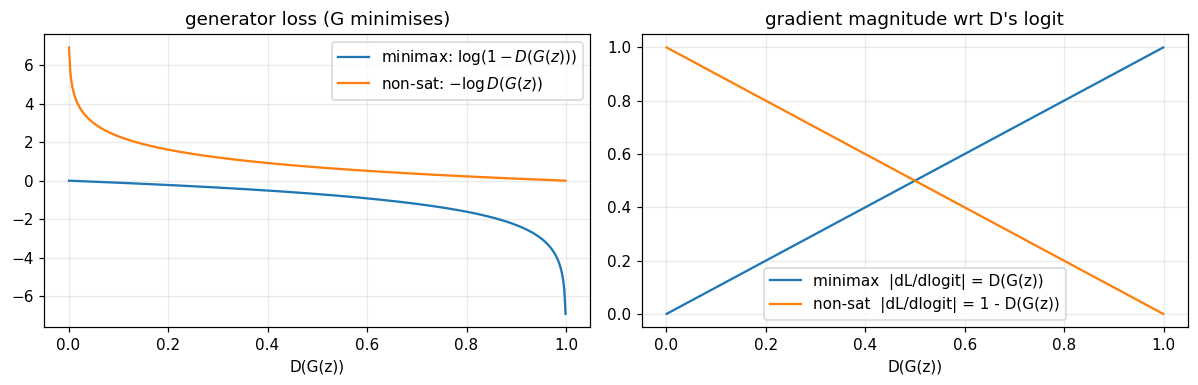
\includegraphics[width=\columnwidth]{figures/fig_loss_saturation.png}
\caption{Generator losses (left) and their gradient magnitude with respect to $D$'s logit (right) as a function of $D(G(z))$. The minimax gradient vanishes exactly where $G$ is weakest.}
\label{fig:sat}
\end{figure}

\subsection{Training procedure}
Each iteration performs $k$ discriminator updates on minibatches of real and generated samples (we use $k=1$ unless stated), followed by one generator update on fresh noise. $D$'s dropout stays active in both steps. A single training loop, parameterized by a configuration object, is used for every experiment so that ablations change exactly one field.

\section{Experimental Setup}
\label{sec:setup}
\subsection{Toy 2-D testbed}
We use two Gaussian mixtures with component standard deviation $\sigma=0.05$: \texttt{ring8} (8 modes on a circle of radius 2) and \texttt{grid25} ($5\times5$ grid with spacing 2). Both networks are 3-layer MLPs with 128 hidden units ($G$: ReLU; $D$: LeakyReLU(0.2)), $z\in\mathbb{R}^2$, Adam ($\beta_1=0.5$, learning rate $5\times10^{-4}$), batch size 256, 5000 iterations. On 5000 generated points we report (a)~\emph{modes covered}: modes receiving at least 10\% of their fair share of high-quality samples; (b)~\emph{hq}: the fraction of samples within $4\sigma$ of some mode; (c)~\emph{JS}: the Jensen--Shannon divergence, normalized to $[0,1]$, between the distribution of high-quality samples over modes and the uniform distribution.

\subsection{MNIST}
We use the standard 50k/10k/10k train/validation/test split of MNIST \cite{lecun1998mnist} with pixels scaled to $[0,1]$ and flattened to 784 dimensions. The generator has $z\in\mathbb{R}^{100}$, two ReLU layers of 1200 units and a sigmoid output; the discriminator has two maxout layers (240 units, 5 pieces) with dropout 0.5. Training uses the non-saturating loss, Adam ($\beta_1=0.5$, lr $2\times10^{-4}$), batch size 100 and 20{,}000 iterations (seed 0). The code is written in PyTorch \cite{paszke2019pytorch} and was run on a CUDA GPU; each 20k-iteration run took under two minutes.

\textbf{Parzen-window metric.} We fit an isotropic Gaussian kernel density estimate on 10{,}000 generated samples, choose $\sigma$ from a 10-point log grid on $[0.1,1]$ by maximizing mean log-likelihood on the validation set, and report the mean log-likelihood on the test set with its standard error across test examples:
\begin{equation}
\log\hat p(x)=\operatorname*{logsumexp}_i\!\Big(-\tfrac{\lVert x-g_i\rVert^2}{2\sigma^2}\Big)-\log N-\tfrac{d}{2}\log(2\pi\sigma^2),
\label{eq:parzen}
\end{equation}
with $d=784$ and $g_i$ the generated samples.

\textbf{Extra diagnostics.} To study collapse we train a small CNN classifier on real MNIST (test accuracy 98.6\%) and compute the class histogram of generated digits, the normalized class entropy (1 means all ten classes equally frequent), and an Inception-style score $\exp(\E_x\mathrm{KL}(p(y|x)\Vert p(y)))$, which is at most 10. On real test data this score is 9.49 and the entropy 0.999.

\subsection{Deviations from the paper}
Our setup differs from the paper in: Adam instead of SGD with momentum; shorter training (20k iterations); a single training seed for the main MNIST run; no re-training of the DBN, CAE and GSN baselines (we quote their numbers); no TFD experiment; and the Parzen $\sigma$ grid of 10 values. Exact numerical agreement is therefore not expected, and the Parzen estimate itself is noisy \cite{theis2016note}.

\section{Results and Discussion}
\label{sec:results}
\subsection{Toy results}
Table~\ref{tab:toy} shows the main comparison over three seeds. On \texttt{ring8} both losses cover essentially all modes. On the harder \texttt{grid25} neither loss covers all 25 modes, and the difference between losses is smaller than the seed-to-seed spread (Figs.~\ref{fig:modes} and~\ref{fig:grid}).

\begin{table}[t]
\caption{Toy results, mean $\pm$ std over 3 seeds (5000 iterations).}
\label{tab:toy}
\centering\small
\setlength{\tabcolsep}{3pt}
\begin{tabular}{llccc}
\toprule
Data & $G$ loss & Modes & hq & JS\\
\midrule
ring8 & minimax & $8.0\pm0.0$ & $0.949\pm0.006$ & $0.001\pm0.000$\\
ring8 & non-sat & $7.7\pm0.6$ & $0.960\pm0.005$ & $0.032\pm0.049$\\
grid25 & minimax & $20.3\pm3.2$ & $0.453\pm0.102$ & $0.150\pm0.074$\\
grid25 & non-sat & $17.7\pm2.5$ & $0.551\pm0.132$ & $0.203\pm0.051$\\
\bottomrule
\end{tabular}
\end{table}

\begin{figure}[t]
\centering
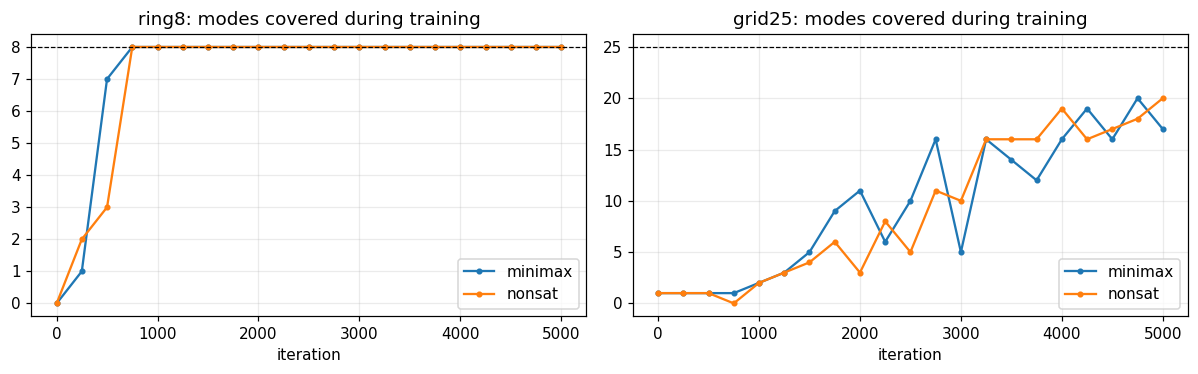
\includegraphics[width=\columnwidth]{figures/fig_modes_over_training.png}
\caption{Number of modes covered during training (seed 0). \texttt{ring8} is solved by both losses within about 750 iterations; \texttt{grid25} improves slowly and noisily towards, but does not reach, 25 modes.}
\label{fig:modes}
\end{figure}

\begin{figure*}[t]
\centering
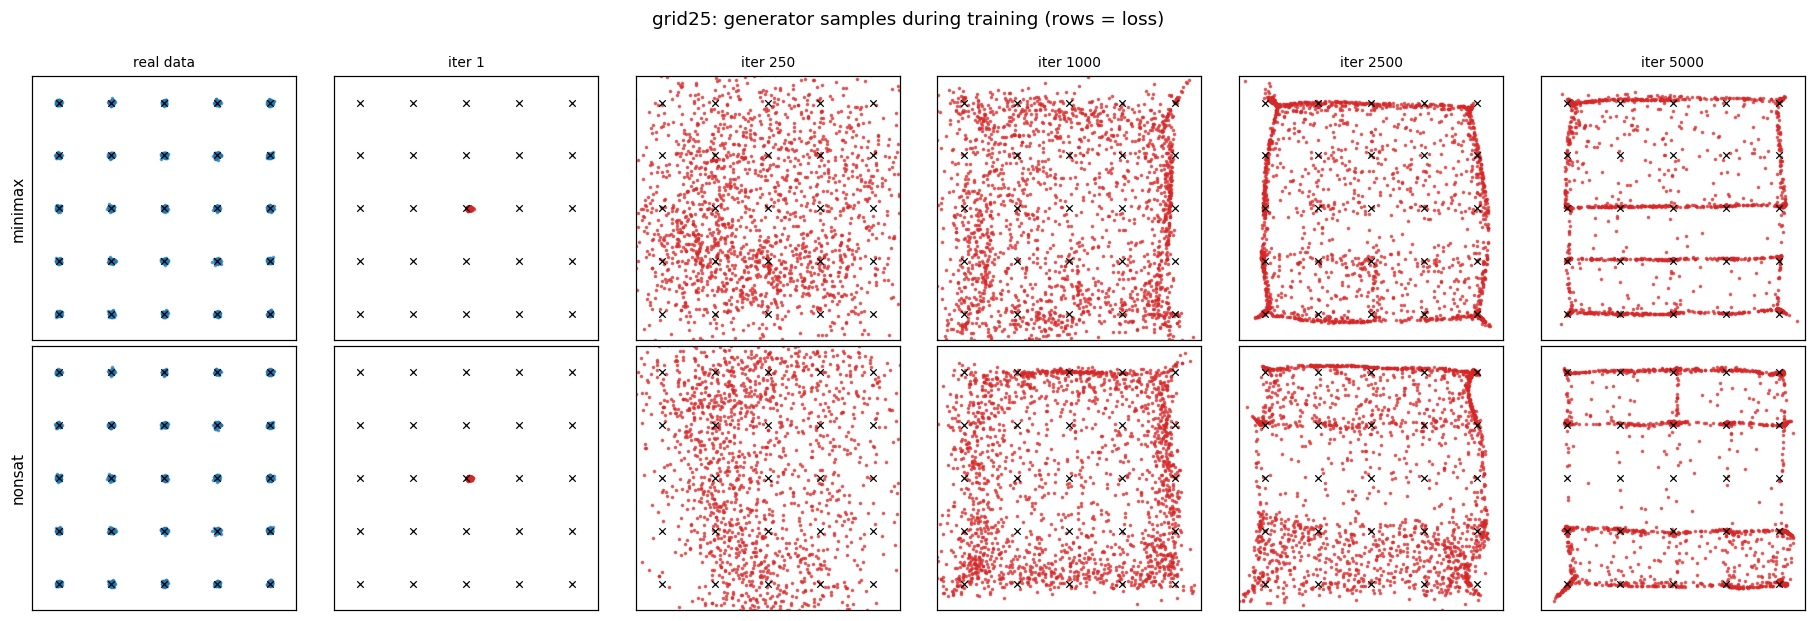
\includegraphics[width=0.85\textwidth]{figures/fig_grid25_snapshots.png}
\caption{Generator samples on \texttt{grid25} during training (seed 0; rows: minimax and non-saturating losses; crosses: true modes). Samples at 5000 iterations lie on lines between modes rather than on the modes, which explains the low high-quality fraction in Table~\ref{tab:toy}.}
\label{fig:grid}
\end{figure*}

\subsection{MNIST: comparison with Table 1 of the paper}
Table~\ref{tab:paper} separates the values quoted from the paper (top) from our own measurements (bottom). Our GAN does not reproduce the paper's result. Both generators collapse: the non-saturating generator outputs one digit ``1'' for every noise vector and the minimax generator outputs a single blob (Figs.~\ref{fig:samples} and~\ref{fig:nn}); the Inception-style score is $\approx1$ and class entropy is near zero. Two reference rows calibrate our estimator: a KDE built from 10k real training images scores $242.4\pm2.1$, close to the paper's 225, while an untrained generator scores $-541.3$. The estimator is therefore working; the generator is not.

\begin{table}[t]
\caption{MNIST Parzen-window log-likelihood (higher is better). Top: values quoted from Table~1 of \cite{goodfellow2014gan}. Bottom: our measurements (seed 0, 20k iterations). IS: Inception-style score (max 10); Ent.: normalized class entropy.}
\label{tab:paper}
\centering\small
\setlength{\tabcolsep}{3pt}
\begin{tabular}{lccc}
\toprule
Model & Log-lik. & IS & Ent.\\
\midrule
DBN [paper] & $138\pm2$ & -- & --\\
Stacked CAE [paper] & $121\pm1.6$ & -- & --\\
Deep GSN [paper] & $214\pm1.1$ & -- & --\\
Adversarial nets [paper] & $225\pm2$ & -- & --\\
\midrule
GAN, non-sat (ours) & $-321.4\pm1.2$ & 1.00 & 0.018\\
GAN, minimax (ours) & $-435.4\pm0.5$ & 1.03 & 0.070\\
KDE of 10k real images & $242.4\pm2.1$ & -- & --\\
Untrained generator & $-541.3\pm0.1$ & 1.00 & --\\
\bottomrule
\end{tabular}
\end{table}

\begin{figure}[t]
\centering
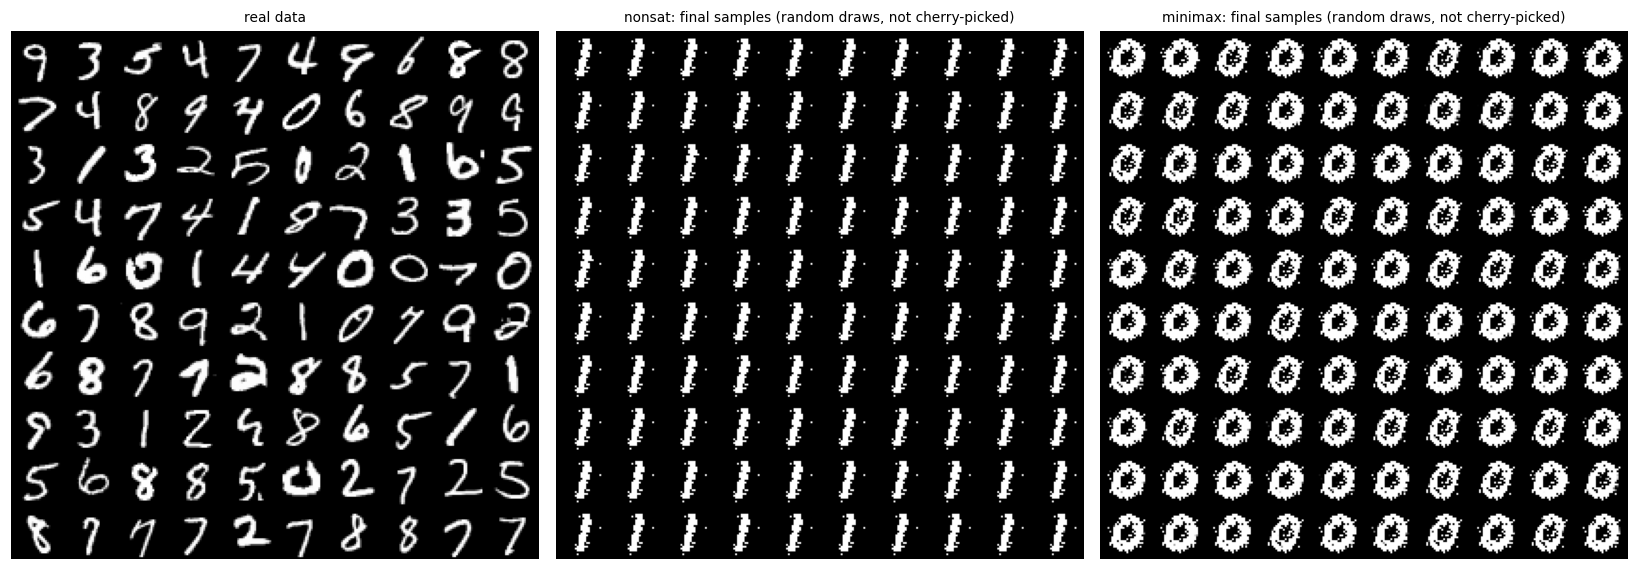
\includegraphics[width=\columnwidth]{figures/fig_mnist_samples.png}
\caption{Real MNIST digits (left) and final samples from our non-saturating (middle) and minimax (right) generators. Both have collapsed. Samples are random draws, not selected.}
\label{fig:samples}
\end{figure}

\begin{figure}[t]
\centering
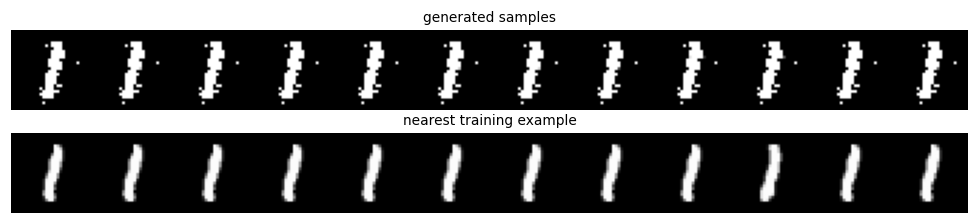
\includegraphics[width=\columnwidth]{figures/fig_mnist_nn_check.png}
\caption{Generated samples (top) and their nearest training images (bottom) for the non-saturating generator, the analogue of Fig.~2 of the paper. Every sample is the same digit, so the check says little about memorization; the median nearest-neighbour distance was 4.59 for generated samples and 4.43 for held-out test images.}
\label{fig:nn}
\end{figure}

\subsection{Why the MNIST run failed}
The training curves (Fig.~\ref{fig:curves}) show that the discriminator wins decisively: mean $D(G(z))$ falls to nearly zero within the first few thousand iterations and $D$'s loss stays near zero. For the minimax loss, the generator's gradient norm decays by many orders of magnitude, as the saturation argument of Sec.~\ref{sec:method} predicts. The non-saturating loss keeps a large gradient yet still collapses, so avoiding saturation alone is not sufficient for stable training in our setup. We did not find a coding error in the losses, but we cannot rule out that our optimizer and capacity choices make $D$ too strong.

\begin{figure*}[t]
\centering
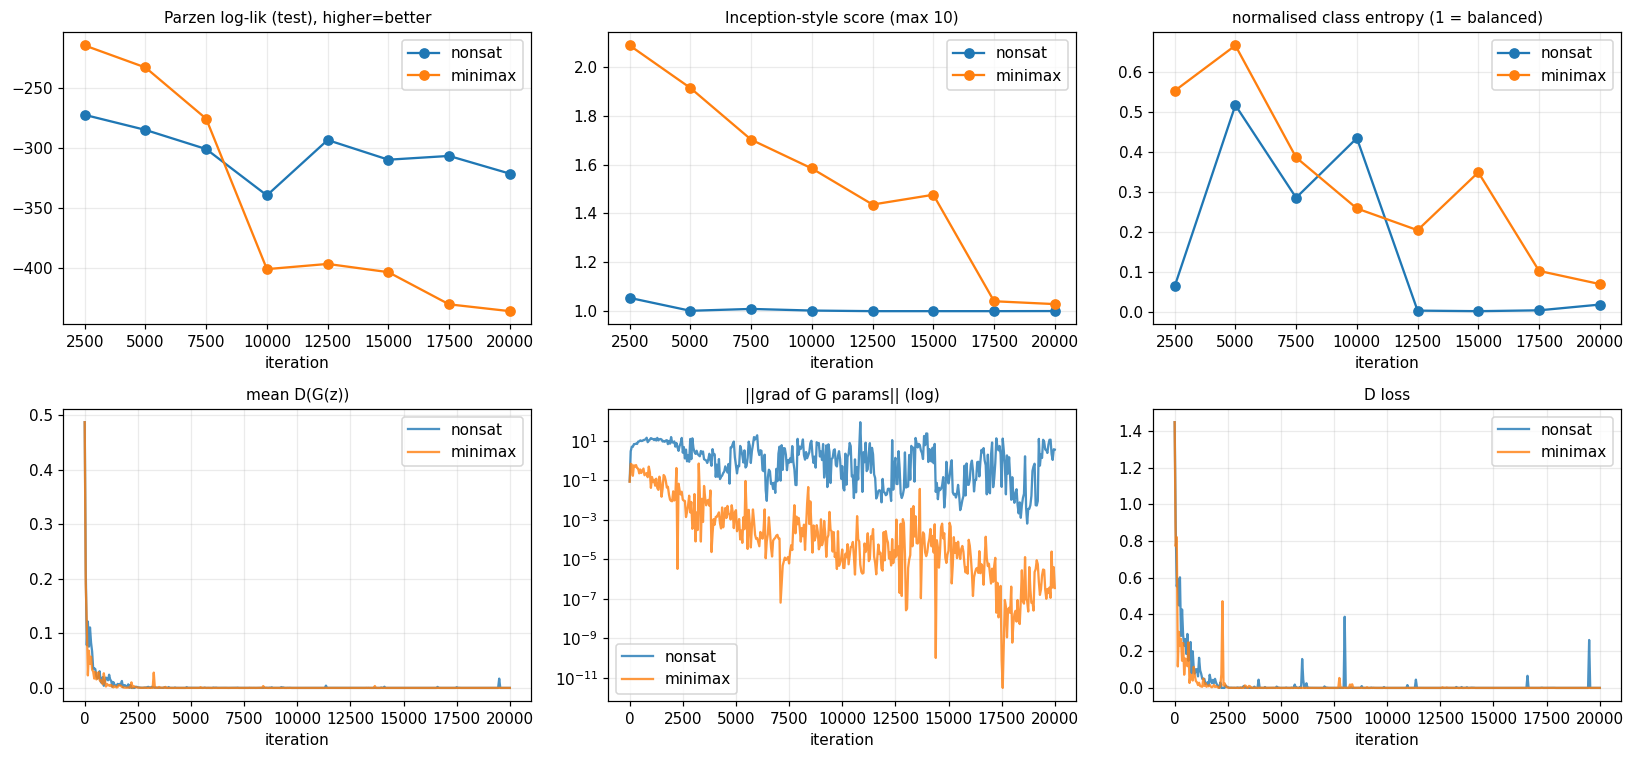
\includegraphics[width=0.85\textwidth]{figures/fig_mnist_curves.png}
\caption{MNIST training diagnostics for both losses (top: Parzen log-likelihood, Inception-style score, class entropy at eight checkpoints; bottom: $D(G(z))$, generator gradient norm, discriminator loss).}
\label{fig:curves}
\end{figure*}

\section{Ablation Study}
\label{sec:ablation}
\subsection{Hypotheses}
\textbf{H1 (loss).} The paper argues that the non-saturating loss gives $G$ a useful gradient where the minimax loss saturates; we therefore expected it to cover more modes or score higher. \textbf{H2 (update ratio).} The paper warns that $G$ must not be trained too much without updating $D$ (the ``Helvetica scenario''); we expected a $G$-heavy ratio to collapse.

\subsection{Toy results}
For H1, Table~\ref{tab:toy} does \emph{not} support an advantage for the non-saturating loss on the toy data: on \texttt{grid25} minimax covers slightly more modes ($20.3\pm3.2$ vs.\ $17.7\pm2.5$), a difference within one standard deviation. A plausible reason, consistent with our diagnostics, is that mean $D(G(z))$ stayed roughly between 0.2 and 0.5 throughout toy training (Fig.~\ref{fig:toydiag}), so the saturating regime was never reached. With only three seeds we treat this as inconclusive rather than as evidence against the paper.

For H2, on \texttt{ring8} (seed 0, non-saturating loss), a $1{:}5$ ratio ($k=1$ discriminator step, 5 generator steps) collapsed to a single point that hops between modes (0/8 modes, JS $=1.0$), while the balanced $1{:}1$ run covered 8/8 modes (Fig.~\ref{fig:helv}). This matches the paper's description. A $5{:}1$ discriminator-heavy ratio gave 2/8 modes by our strict metric (hq 0.93, JS 0.50); the samples trace the circle but fail to settle on modes. In the larger \texttt{grid25} ablation (2 seeds) the $1{:}5$ ratio also collapsed (0.5 and 1.5 modes for minimax and non-saturating, respectively).

\begin{figure}[t]
\centering
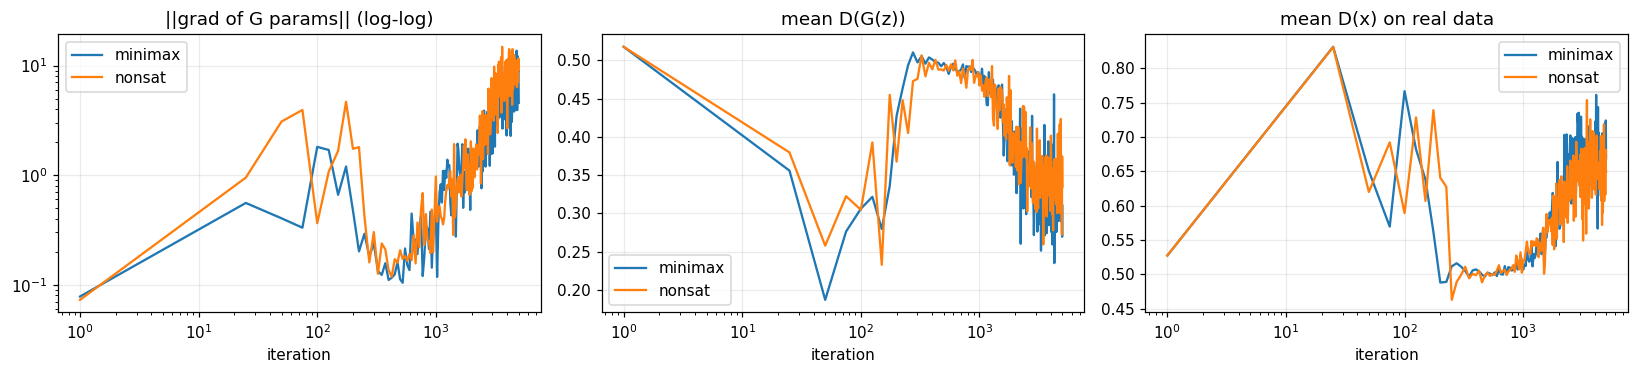
\includegraphics[width=\columnwidth]{figures/fig_toy_diagnostics.png}
\caption{Toy (\texttt{grid25}) diagnostics: generator gradient norm, mean $D(G(z))$ and mean $D(x)$. Mean $D(G(z))$ stays well above zero.}
\label{fig:toydiag}
\end{figure}

\begin{figure*}[t]
\centering
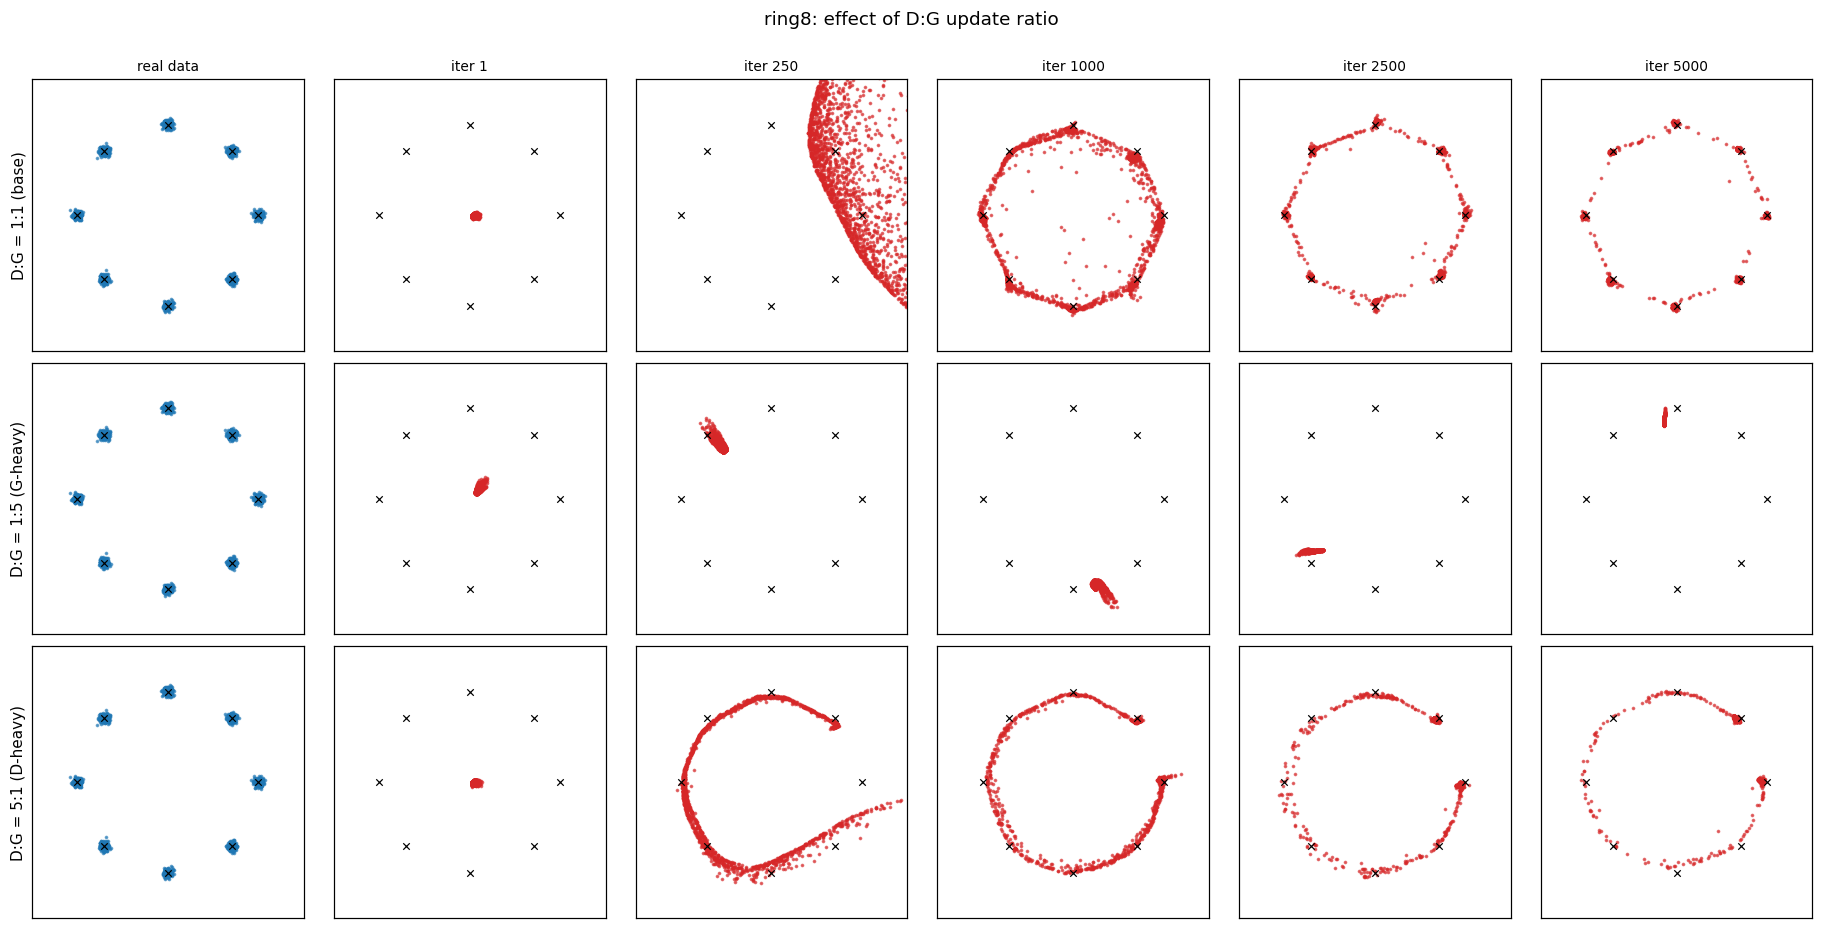
\includegraphics[width=0.8\textwidth]{figures/fig_helvetica.png}
\caption{Effect of the $D{:}G$ update ratio on \texttt{ring8} (seed 0, non-saturating loss). Red: generated samples; crosses: true modes. The $G$-heavy run collapses to a point, as in the paper's ``Helvetica scenario''.}
\label{fig:helv}
\end{figure*}

\subsection{MNIST ablation (preliminary)}
Table~\ref{tab:mnabl} varies one factor at a time from the base configuration, trained for 8000 iterations with a \emph{single seed}. Because the base configuration itself is collapsed (score 1.00), these numbers should be read only as leads. Two changes stand out: reducing the noise dimension from 100 to 10 gave a Parzen log-likelihood of $+103.9$ with score 5.87 and entropy 0.89, and a narrower generator (128 units) gave $-131.1$ with score 1.94. Every other change left the score near 1. Without repeated seeds we cannot say whether these gains are robust.

\begin{table}[t]
\caption{MNIST one-factor ablation, 8000 iterations, \emph{one seed} (preliminary). Base: non-sat loss, $z{=}100$, $G$ width 1200, dropout 0.5, maxout $D$, $D{:}G=1{:}1$, Adam $\beta_1{=}0.5$.}
\label{tab:mnabl}
\centering\small
\setlength{\tabcolsep}{3pt}
\begin{tabular}{llccc}
\toprule
Factor & Setting & Log-lik. & IS & Ent.\\
\midrule
-- & base & $-295.1$ & 1.00 & 0.004\\
Loss & minimax & $-410.1$ & 1.02 & 0.051\\
$D$ dropout & 0.0 & $-445.0$ & 1.01 & 0.227\\
$D$ activation & leaky ReLU & $-350.1$ & 1.01 & 0.287\\
$D{:}G$ steps & $3{:}1$ & $-546.9$ & 1.00 & 0.005\\
$D{:}G$ steps & $1{:}3$ & $-331.6$ & 1.00 & 0.113\\
$z$ dim & 10 & $\mathbf{103.9}$ & 5.87 & 0.894\\
$G$ width & 512 & $-524.3$ & 1.00 & 0.059\\
$G$ width & 128 & $-131.1$ & 1.94 & 0.466\\
Adam $\beta_1$ & 0.0 & $-796.9$ & 1.00 & 0.032\\
Adam $\beta_1$ & 0.9 & $-682.2$ & 1.00 & 0.597\\
\bottomrule
\end{tabular}
\end{table}

\section{Limitations and Failure Cases}
\label{sec:limits}
\begin{itemize}
\item \textbf{Failed reproduction.} Our MNIST GAN collapsed (Sec.~\ref{sec:results}); the $-321$ vs.\ $+225$ comparison is not a valid reproduction of the paper's claim, only a record of a failed attempt.
\item \textbf{Few seeds.} The main MNIST run and the whole MNIST ablation use one seed; the toy ablation uses two or three. GANs are noisy, so small differences are not reliable.
\item \textbf{Optimizer and training length.} We use Adam and 20k iterations rather than the paper's SGD with momentum, and we did not tune the base MNIST configuration on the validation set before running ablations.
\item \textbf{Metric weakness.} The Parzen estimator has high variance and is unreliable in 784 dimensions \cite{goodfellow2014gan,theis2016note}. The $+103.9$ result in Table~\ref{tab:mnabl} should not be compared to 225 without repeated runs.
\item \textbf{Scope.} We did not retrain the DBN, CAE or GSN baselines and did not attempt the TFD or CIFAR-10 experiments. Our mode-coverage metric on the toy data depends on the $4\sigma$ and 10\% thresholds we chose.
\end{itemize}

\section{Conclusion and Future Work}
We implemented the GAN objective, a maxout discriminator and the Parzen evaluation pipeline from scratch and verified the paper's qualitative warning about unbalanced updates on a toy problem. We could not reproduce the paper's MNIST Parzen result: both of our generators collapsed, with the discriminator overpowering the generator. A reduced noise dimension or generator width looks like a promising fix, but this is a single-seed observation. Future work is to select the base configuration using only validation data, run at least three seeds, and repeat the loss ablation on a healthy MNIST baseline before drawing conclusions about H1.

\section*{Code and Attribution}
All model, loss and training code was written by the author for this project using standard PyTorch layers, optimizers and the torchvision MNIST loader. No third-party GAN implementation is reproduced here.

\bibliographystyle{IEEEtran}
\bibliography{references}

\end{document}
